\documentclass[11pt,a4paper]{article}

\usepackage[T1]{fontenc}
\usepackage[utf8]{inputenc}
\usepackage[margin=2.4cm]{geometry}
\usepackage{lmodern}
\usepackage{amsmath,amssymb}
\usepackage{listings}
\usepackage{xcolor}
\usepackage{enumitem}
\usepackage{fancyhdr}
\usepackage{tikz}
\usetikzlibrary{shapes.geometric,arrows.meta,positioning}
\usepackage[hidelinks]{hyperref}
\usepackage{microtype}
% Command-line flags must render as two hyphens, not an en-dash.
\DisableLigatures[-]{encoding=T1,family=tt*}

\definecolor{codebg}{gray}{0.96}
\definecolor{codekw}{RGB}{20,80,160}
\definecolor{codecm}{RGB}{100,110,100}
\definecolor{codestr}{RGB}{150,60,20}

\lstdefinestyle{src}{
  backgroundcolor=\color{codebg},
  basicstyle=\ttfamily\footnotesize,
  keywordstyle=\color{codekw}\bfseries,
  commentstyle=\color{codecm}\itshape,
  stringstyle=\color{codestr},
  showstringspaces=false,
  columns=fullflexible,
  keepspaces=true,
  breaklines=true,
  frame=leftline,
  framerule=1.2pt,
  rulecolor=\color{codekw!40},
  xleftmargin=10pt,
  framexleftmargin=8pt,
  aboveskip=8pt,
  belowskip=8pt,
  literate={°}{{\textdegree}}1,
}
\lstdefinestyle{sh}{style=src,language=bash,morekeywords={esbmc,ltl2ba}}
\lstset{style=src,language=C}

\newcommand{\esbmc}{ESBMC}
\newcommand{\flag}[1]{\texttt{\small #1}}
\newcommand{\file}[1]{\texttt{\small #1}}

\newlist{parts}{enumerate}{1}
\setlist[parts]{label=(\alph*), leftmargin=2em, topsep=4pt, itemsep=3pt}

\newcounter{exc}
\newenvironment{exercise}[1]
  {\stepcounter{exc}\medskip\noindent\textbf{\theexc) (#1)}\par\nopagebreak\smallskip}
  {\par\medskip}

\pagestyle{fancy}
\fancyhf{}
\lhead{\small Specification and Verification of Embedded and Cyber-Physical Systems}
\rhead{\small \thepage}
\renewcommand{\headrulewidth}{0.4pt}

\emergencystretch=3em

\title{\vspace{-1.5cm}Specification and Verification of\\Embedded and Cyber-Physical Systems\\[4pt]
       \large Exercises --- \esbmc{} 8.5}
\author{}
\date{}

\begin{document}
\maketitle
\vspace{-1.6cm}

\section*{Before you start}

Every command below was run against \esbmc{} \textbf{8.5.0}, and the sources are
in \file{exercises/ecps/}. The LTL exercises additionally need
\href{https://github.com/esbmc/libltl2ba}{libltl2ba}, the ESBMC fork of
\texttt{ltl2ba}; the upstream \texttt{ltl2ba} shipped by Homebrew and most
distributions has no \flag{-O c} backend and cannot produce an \esbmc{} monitor.

\begin{lstlisting}[style=sh]
esbmc --version                                   # expect 8.5.0 or newer
git clone https://github.com/esbmc/libltl2ba.git && make -C libltl2ba
cd exercises/ecps && ./run-all.sh                 # every verdict below
\end{lstlisting}

\noindent
\textbf{The one thing that catches everybody.} \esbmc{} does \emph{not} negate
your LTL formula for you. The polarity you hand \texttt{ltl2ba} is the question
you are asking:

\smallskip
\begin{center}
\begin{tabular}{@{}lll@{}}
\texttt{\small -f '!G(...)'} & does the property \emph{hold} here?
  & \texttt{\small LTL\_SUCCEEDING} $\Rightarrow$ SUCCESSFUL \\
\texttt{\small -f 'G(...)'}  & can it be \emph{refuted} here?
  & \texttt{\small LTL\_FAILING} $\Rightarrow$ FAILED \\
\end{tabular}
\end{center}
\smallskip

\noindent
Use the negated form when you are asking whether a controller is correct. When
you report a verdict, say which polarity produced it.

\section{Bounded model checking}

\begin{exercise}{Bounded Model Checking}
Describe the steps involved in checking a program with the BMC technique, from
reading the program to generating the SMT formulas. Use the actuator ramp below
to describe each step: the heater duty cycle rises by a fixed increment on every
tick of the control loop. \texttt{\_\_ESBMC\_assume} constrains
(non-deterministic) variables and \texttt{assert} states the property to check.

\begin{lstlisting}
/* exercises/ecps/ramp.c */
#include <assert.h>
#define STEP 2                    /* duty increment per tick */

int main(int argc, char **argv) {
  long long int tick = 1, duty = 0;
  unsigned int ticks = 5;         /* ticks in this ramp */
  __ESBMC_assume(ticks >= 1);
  while (tick <= ticks) {
    duty = duty + STEP;
    tick++;
  }
  assert(duty == ticks * STEP);
}
\end{lstlisting}

\begin{parts}
  \item Unroll the loop by hand for \texttt{ticks = 5} and write the resulting
        single-assignment (SSA) form.
  \item Split the SSA form into the constraint $C$ and the property $P$, and
        give the formula the solver is asked to decide. Which answer ---
        \emph{satisfiable} or \emph{unsatisfiable} --- corresponds to
        \texttt{VERIFICATION FAILED}?
  \item Run \texttt{esbmc ramp.c}. Compare the assignment count reported by
        \emph{Symex completed} with the number surviving \emph{Slicing}. What
        did the slicer remove, and why is removing it sound?
  \item Replace \texttt{ticks = 5} with \texttt{ticks = nondet\_uint()} and run
        \texttt{esbmc ramp.c --unwind 6}. Explain what \flag{--unwind} now
        controls and what a failing \emph{unwinding assertion} is telling you.
  \item The same control loop in Python is
        \file{exercises/ecps/settle.py}: the heater ramps in fixed 2-degree
        steps until the measured temperature equals the setpoint.

\begin{lstlisting}[language=Python]
def settle(setpoint: int) -> int:
    temp = 0
    while temp != setpoint:
        temp = temp + 2
    return temp

settle(10)  # reachable in 5 ticks
settle(7)   # unreachable: an odd setpoint is never hit in steps of 2
\end{lstlisting}

        Run \texttt{esbmc settle.py --unwind 8}. Explain what a bounded model
        checker can and cannot tell you about termination here, and state the
        precondition on \texttt{setpoint} that makes the loop terminate.
\end{parts}
\end{exercise}

\section{Concurrency and mutual exclusion}

\begin{exercise}{Race condition on the display bus}
The T and P tasks hand their samples to the S task over a single-word display
bus, and only one task may drive the bus at a time. \file{ecps/bus.c}
arbitrates with Peterson's algorithm; \texttt{in\_T} and \texttt{in\_P} record
which task currently owns the bus.

\begin{lstlisting}
/* exercises/ecps/bus.c */
void *task_T(void *arg) {              void *task_P(void *arg) {
  want[0] = 1;                           want[1] = 1;
  turn = 1;                              turn = 0;
  while (want[1] && turn == 1) {}        while (want[0] && turn == 0) {}
  in_T = 1;                              in_P = 1;
  bus_word = 1;  /* temperature */       bus_word = 2;  /* pressure */
  in_T = 0;                              in_P = 0;
  want[0] = 0;                           want[1] = 0;
  return 0;                              return 0;
}                                      }
\end{lstlisting}

\begin{parts}
  \item Specify the following three properties in LTL, using $c_i$ for ``task
        $i$ is driving the bus'' ($\texttt{in\_T}$, $\texttt{in\_P}$) and $r_i$
        for ``task $i$ has requested the bus'' ($\texttt{want[0]}$,
        $\texttt{want[1]}$).
        \begin{enumerate}[label=\roman*.,leftmargin=2.2em,topsep=2pt]
          \item At most one task is driving the bus at any time.
          \item Whenever a task requests the bus, it eventually gets it.
          \item A task can eventually request the bus.
        \end{enumerate}
  \item Which are \emph{safety} properties and which are \emph{liveness}
        properties? Which can a bounded run refute, and which can it only fail
        to refute?
  \item Verify property (i) with \esbmc{}. Generate the monitor and run it:

\begin{lstlisting}[style=sh]
ltl2ba -O c -H '"bus.h"' -f '!G(!({in_T} && {in_P}))' > bus-mutex-neg.ba-2.c
esbmc bus.c --ltl bus-mutex-neg.ba-2.c -DLTL_PREFIX_BOUND=10 --context-bound 3
\end{lstlisting}

        Report the \emph{Final lowest outcome}.
  \item Now break the algorithm: delete \texttt{turn = 1;} from
        \texttt{task\_T} and re-run the same monitor. The outcome changes to
        \texttt{LTL\_BAD}, not \texttt{LTL\_FAILING}. Explain the difference
        between the two, and give the interleaving that puts both tasks on the
        bus at once.
  \item Encode property (ii) and check it. A bounded run cannot establish it ---
        say what verdict you get and why that is the expected answer rather
        than a tool limitation.
\end{parts}
\end{exercise}

\section{Specifying and verifying an embedded system}

\begin{exercise}{Cyber-threats and control properties}
A typical embedded system consists of a \emph{human--machine interface}
(keyboard and display), a \emph{processing unit} (real-time computer system),
and an \emph{instrumentation interface} (sensor, network, and actuator) that can
be connected to some physical plant. Figure~\ref{fig:plant} illustrates a simple
embedded system employed in a chemical process, which can be operated remotely
via TCP/IP. It contains two Analog-to-Digital Converters (ADC) and a
Digital-to-Analog Converter (DAC). The first ADC reads the thermocouples'
temperature; the second reads the pressure transducer. The DAC sets the desired
position of the valve/pump, and a switch turns the heater on or off. The overall
objective is to keep the temperature and pressure of the chemical process within
well-defined limits, under a remote operator.

\begin{figure}[htbp]
\centering
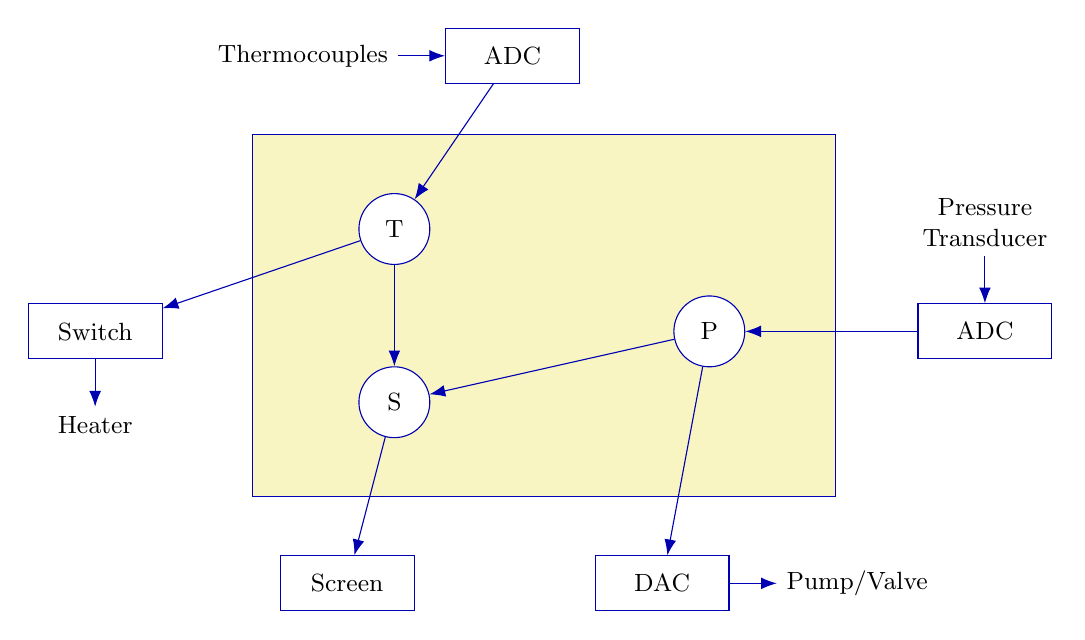
\begin{tikzpicture}[
  font=\small,
  box/.style={draw=blue!70!black, fill=white, minimum width=17mm, minimum height=7mm},
  proc/.style={draw=blue!70!black, fill=white, circle, minimum size=9mm},
  ar/.style={-{Latex[length=2mm]}, draw=blue!70!black},
]
\fill[black!12!yellow!25, draw=blue!70!black] (0,0) rectangle (7.4,4.6);
\node[proc] (T) at (1.8,3.4) {T};
\node[proc] (P) at (5.8,2.1) {P};
\node[proc] (S) at (1.8,1.2) {S};

\node[box] (adcT) at (3.3,5.6) {ADC};
\node[box] (adcP) at (9.3,2.1) {ADC};
\node[box] (sw)   at (-2.0,2.1) {Switch};
\node[box] (scr)  at (1.2,-1.1) {Screen};
\node[box] (dac)  at (5.2,-1.1) {DAC};

\node[left=6mm of adcT, align=right] (tc) {Thermocouples};
\node[above=6mm of adcP, align=center] (pt) {Pressure\\Transducer};
\node[below=6mm of sw] (heat) {Heater};
\node[right=6mm of dac] (pv) {Pump/Valve};

\draw[ar] (tc) -- (adcT);
\draw[ar] (adcT) -- (T);
\draw[ar] (pt) -- (adcP);
\draw[ar] (adcP) -- (P);
\draw[ar] (T) -- (sw);
\draw[ar] (sw) -- (heat);
\draw[ar] (T) -- (S);
\draw[ar] (P) -- (S);
\draw[ar] (S) -- (scr);
\draw[ar] (P) -- (dac);
\draw[ar] (dac) -- (pv);
\end{tikzpicture}
\caption{Simple embedded system [7].}
\label{fig:plant}
\end{figure}

\file{exercises/ecps/plant.c} implements this system as a cyclic executive: each
round runs T, P and then S. The two ADC readings are non-deterministic within
their transducer ranges, so one \esbmc{} run covers every reading the hardware
can produce.

\begin{lstlisting}
/* exercises/ecps/plant.c -- abridged */
static void process_T(void) {                 /* temperature control */
  temperature = read_thermocouple();          /* nondet, -50..400 degC */
  if (temperature < TEMP_LOW)       heater_on = 1;
  else if (temperature > TEMP_HIGH) heater_on = 0;
}
static void process_P(void) {                 /* pressure control */
  pressure = read_transducer();               /* nondet, 0..600 bar */
  if (pressure > PRESS_HIGH)     valve_open = 1;
  else if (pressure < PRESS_LOW) valve_open = 0;
}
static void process_S(void) {                 /* screen refresh */
  if (fresh_sample && !bus_busy()) { displayed = 1; fresh_sample = 0; }
}
\end{lstlisting}

\begin{parts}
  \item Specify the following properties of this embedded system using LTL. The
        propositions available to the monitor are declared in \file{plant.h}:
        \texttt{temperature}, \texttt{pressure}, \texttt{heater\_on},
        \texttt{valve\_open}, \texttt{fresh\_sample} and \texttt{displayed}.
        \begin{enumerate}[label=\alph*.,leftmargin=2.2em,topsep=2pt]
          \item A T process reads the measured values from a temperature sensor,
                turns the heating system on if the temperature is below
                20\,\textdegree C, and turns off the heating system if the
                temperature is above 300\,\textdegree C.
          \item Process P regulates pressure with a sensor opening the pump/valve
                when the pressure value is above 500\,bar and closing the
                pump/valve when the pressure value is below 100\,bar.
          \item The measured values will be shown on a liquid crystal display
                (LCD) when the T and P processes transfer data to an S process.
        \end{enumerate}
  \item Verify each of your three formulas with \esbmc{}. Generate the monitor
        from the \emph{negated} formula, since you are asking whether the
        property holds:

\begin{lstlisting}[style=sh]
ltl2ba -O c -H '"plant.h"' -f '!G({pressure > 500} -> F {valve_open})' \
       > valve-neg.ba-2.c
esbmc plant.c --ltl valve-neg.ba-2.c -DLTL_PREFIX_BOUND=10
\end{lstlisting}

        Exactly one of the three reports
        \texttt{VERIFICATION SUCCESSFUL}. Report all three outcomes.
  \item The heater property fails. Read the counterexample and find the defect.
        \emph{Hint:} look at the value of \texttt{temperature} before the first
        round runs, and at what the specification therefore requires of the
        controller at that instant. Why does the pressure property not have the
        same problem?
  \item Repair \file{plant.c} so the heater property holds, re-verify, and state
        what your repair assumes about the hardware.
  \item The screen property also fails, for an entirely different reason.
        Diagnose it, and say what assumption about the display bus you would
        have to add --- and how you would express it --- for the property to
        become provable.
  \item What are the \textbf{security objectives} of this simple embedded
        system?
  \item What are the sources of security problems that can arise when this
        system is operated remotely? Consider the TCP interface specifically,
        and say which of your LTL properties would still hold if an attacker
        could set \texttt{heater\_on} directly.
\end{parts}
\end{exercise}

\section*{References}

\sloppy
\begin{enumerate}[leftmargin=2.4em,itemsep=3pt,label={[\arabic*]}]
  \item L. C. Cordeiro, B. Fischer, J. Marques-Silva. ``SMT-Based Bounded Model
        Checking for Embedded ANSI-C Software''. \emph{IEEE Transactions on
        Software Engineering} 38(4):957--974, 2012.
        \href{https://doi.org/10.1109/TSE.2011.59}{doi:10.1109/TSE.2011.59}
  \item M. Y. R. Gadelha, H. I. Ismail, L. C. Cordeiro. ``Handling loops in
        bounded model checking of C programs via k-induction''.
        \emph{International Journal on Software Tools for Technology Transfer}
        19(1):97--114, 2017.
        \href{https://doi.org/10.1007/s10009-015-0407-9}{doi:10.1007/s10009-015-0407-9}
  \item M. Y. R. Gadelha, F. R. Monteiro, J. Morse, L. C. Cordeiro, B. Fischer,
        D. A. Nicole. ``ESBMC 5.0: an industrial-strength C model checker''.
        \emph{ASE 2018}, pp. 888--891.
        \href{https://doi.org/10.1145/3238147.3240481}{doi:10.1145/3238147.3240481}
  \item B. Farias, R. Menezes, E. B. de Lima Filho, Y. Sun, L. C. Cordeiro.
        ``ESBMC-Python: A Bounded Model Checker for Python Programs''.
        \emph{ISSTA 2024}, pp. 1836--1840.
        \href{https://doi.org/10.1145/3650212.3685304}{doi:10.1145/3650212.3685304}
  \item N. Tihanyi, Y. Charalambous, R. Jain, M. A. Ferrag, L. C. Cordeiro.
        ``A New Era in Software Security: Towards Self-Healing Software via
        Large Language Models and Formal Verification''. \emph{AST@ICSE 2025},
        pp. 136--147.
        \href{https://doi.org/10.1109/AST66626.2025.00020}{doi:10.1109/AST66626.2025.00020}
  \item C. Baier, J.-P. Katoen. \emph{Principles of Model Checking}. MIT Press,
        2008. ISBN 978-0-262-02649-9.
  \item A. Burns, A. J. Wellings. \emph{Real-Time Systems and Programming
        Languages: Ada, Real-Time Java and C/Real-Time POSIX}, 4th edition.
        Addison-Wesley, 2009. ISBN 978-0-321-41745-9. Source of the
        chemical-process case study in Figure~\ref{fig:plant}.
\end{enumerate}

\end{document}
